\documentclass[a4paper,12pt]{article}

\usepackage{mystyle}
\usepackage{gensymb}

\graphicspath{ {images/} }

\definecolor{my-red}{RGB}{139, 0, 139}
\definecolor{my-blue}{RGB}{0, 0, 204}
\definecolor{my-cyan}{RGB}{1, 121, 126}

\newtheorem{proposition}{Утверждение}[section]


\author{Алексеев Василий}


\title{Семинар 10 + 11}
\date{17 + 21 + 24 + 28 ноября 2022}


\begin{document}
  \maketitle
  
  \tableofcontents

  \thispagestyle{empty}
  
  \newpage
  
  \pagenumbering{arabic}


  \section{Аффинные преобразования плоскости}
  
  \subsection{Про отображения}
  
  Отображение $f$ из $\mathcal X$ в $\mathcal Y$~---~это закон, по которому элементу $x \hm\in \mathcal X$ ставится в соответствие элемент $y \hm\in \mathcal Y$.
  Область определения функции $f$~---~это подмножество элементов $D_f \hm\subseteq \mathcal X$, на которых функция определена\footnote{$D_f$~---~одно из возможных обозначений области определения, есть и другие.}.
  Область значений функции $f$~---~это образ области значений $D_f$, то есть $\{y \hm\in \mathcal Y \hm\mid \exists x \hm\in \mathcal X\colon f(x) \hm= y\}$.
  
  Дадим ещё пару определений, касающихся свойств отображений.
  
  \begin{definition}[Инъекция]
    Функция \emph{инъективна}, если разные элементы $\mathcal X$ под действием функции $f$ переводятся в разные элементы $\mathcal Y$:
    \[
      x_1, x_2 \in \mathcal X,\ x_1 \not= x_2 \Rightarrow f(x_1) \not= f(x_2)
    \]
  \end{definition}
  
  \begin{definition}[Сюръекция]
    Функция \emph{сюръективна}, если для любого элемента из $\mathcal Y$ существует прообраз:
    \[
      \forall y \in \mathcal Y \exists x \in \mathcal X\colon f(x) = y
    \]
  \end{definition}
  
  \begin{definition}[Биекция]
    Функция \emph{биективна}, если для любого элемента из $\mathcal Y$ существует единственный прообраз, то есть если функция инъективна и сюръективна.
  \end{definition}
  
  \begin{definition}[Композиция отображений]
    Пусть есть отображения $f\colon \mathcal X \hm\to \mathcal Y$ и $g\colon \mathcal Y \hm\to \mathcal Z$, причём $f(X) \hm\subseteq D_g \hm\subseteq Y$.
    Тогда композицией\footnote{Автор конспекта не смог выяснить, является ли порядок слов важным при обозначении композиции или нет. Например, одно ли то же ``композиция $f$ и $g$'' и ``композиция $g$ и $f$''? Кажется, в русском языке на словах порядок отображений в композиции не выражается, только в виде формулы...} отображений $f$ и $g$ называется отображение $h\colon \mathcal X \hm\to \mathcal Z$, такое что
    \[
      h(x) = g(f(x))
    \]
    
    Отображение $h$ может обозначаться как $g\circ f$ или $gf$\footnote{Хотя иногда под обозначением $gf$ могут иметь в виду \href{https://en.wikipedia.org/wiki/Function\_composition\#Alternative\_notations}{``обратный'' порядок применения отображений}.}.
  \end{definition}

  \begin{theorem}
    Любая функция $f\colon \mathcal X \hm\to \mathcal Y$ может быть представлена как композиция сюръекции, биекции и инъекции.\footnote{Кто первым сформулировал и доказал это утверждение~---~автор конспекта не в курсе. Но, тем не менее, считает нелишним сослаться на работу Рудакова~К.~В. \href{https://yourcmc.ru/wiki/images/1/15/RudakovDocDisser.pdf}{\emph{Алгебраическая теория универсальных и локальных ограничений для алгоритмов распознавания}} (ВЦ~РАН, 1992). Так как именно на семинарах, посвящённых, в сущности, разбору указанной работы, автор конспекта и познакомился с приводимым утверждением о возможности разложения произвольной функции в композицию.}
  \end{theorem}
  
  \begin{proof}
    \begin{figure}
      \centering
      
      \includegraphics[width=0.8\columnwidth]{tribute-to-algebraic-approach}
      
      \caption{Любое отображение $f$ можно представить как композицию отображений.}
      \label{fig:tribute-to-algebraic}
    \end{figure}
    
    Пусть $\alpha\colon \mathcal X \hm\to \mathcal X|_f$~---~функция, которая каждый элемент $x \hm\in \mathcal X$ переводит в подмножество элементов $S(x) \hm\subseteq \mathcal X$, такое что $\forall x' \hm\in \mathcal X\colon f(x') \hm= f(x) \hm\Rightarrow x' \hm\in S(x)$.
    А $\mathcal X|_f$~---~множество таких подмножеств из $\mathcal X$, на которых значение функции $f$ одинаково.
    Очевидно, отображение $\alpha$ сюръективно.
    
    Пусть $\beta\colon \mathcal X|_f \hm\to f(\mathcal X)$~---~отображение, которое каждый элемент $S \hm\in \mathcal X|_f$ переводит в значение функции $f$ на элементе $x \hm\in S$.
    По построению $\mathcal X|_f$, не важно, какой элемент выбрать из $S$ для вычисления значения функции $f$.
    Очевидно, отображение $\beta$ биективно.
    
    Пусть $\gamma\colon f(\mathcal X) \hm\to \mathcal Y$~---~тождественное отображение, то есть $\gamma(y) \hm= y$, $\forall y \hm\in f(\mathcal X)$.
    Очевидно, $\gamma$~---~инъективное отображение.
    
    Таким образом, $f \hm= \gamma \circ \beta \circ \alpha$~(см. рисунок~\ref{fig:tribute-to-algebraic}).
  \end{proof}
  
  
  \subsection{Про линейные преобразования}
  
  Перейдём к случаю отображений из одной плоскости в другую $f\colon P \hm\to Q$.
  Даже в более частному случаю отображений из плоскости в ту же плоскость $f\colon P \hm\to P$, которые ещё называют \emph{преобразованиями}.
  
  \begin{remark}
    Смысл ``преобразования'' в том, что \emph{все} точки плоскости переходят в какие-то (возможно, другие) точки той же плоскости.
    То есть область определения преобразования плоскости~---~это вся плоскость.
    Поэтому далее про ``область определения'' больше вспоминать не будем.
  \end{remark}
  
  Примерами преобразований плоскости могут служить поворот, параллельный перенос, симметрия относительно оси или точки, гомотетия\footnote{Гомотетия с центром в точке $O$ и коэффициентом $k \hm> 0 $ каждой точке $M$ ставит в соответствие точку $M^\star$, так что $\vv{OM^\star} \hm= k\vv{OM}$}.
  % TODO: pic
  
  Преобразования плоскости тоже могут быть инъективными, сюръективными, биективными.
  Например, отображение всех точек плоскости в одну и ту же точку не является ни инъективным, ни сюръективным отображением.
  Можно привести пример инъективного отображения плоскости в круг\footnote{
    Например, круг с центром в начале координат.
    Каждую точку $M$ плоскости можно взаимно однозначно перевести в точку круга: через $M$ и начало координат можно провести прямую $l$ и рассмотреть часть этой прямой внутри круга (отрезок).
    Известно, что отрезок равносилен всей числовой прямой, поэтому между отрезком и прямой $l$ можно установить взаимно однозначное соответствие, и точка $M$ при этом перейдёт в какую-то точку отрезка.
  }.
  В качестве сюръективного отображения можно, например, в некоторой декартовой системе координат на плоскости взять отображение
  \[
    (x, y) \mapsto \left(x^2 - y^2, 2xy\right)
  \]
  
  В последнем примере мы обратились к координатной записи преобразования.
  Преобразование (и вообще отображение) переводит точку в точку.
  Поэтому, выбрав систему координат на плоскости, закон сопоставления точек можно выразить через их координаты, указав, как вычислять положение $x^*$ и $y^*$ точки-образа.
  
  \begin{definition}
    \emph{Линейным} называется преобразование, которое в некоторой декартовой системе координат можно выразить формулами
    \begin{equation}
      \label{eq:linear}
      \left\{
        \begin{aligned}
          &x^\star = a_1 x + b_1 y + c_1\\
          &y^\star = a_2 x + b_2 y + c_2
        \end{aligned}
      \right.
    \end{equation}
    
    При этом $a_i, b_i, c_i \hm\in \RR,\ i = 1, 2$.
  \end{definition}
  
  \begin{example}
    Линейным, очевидно, будет следующее преобразование~(\ref{fig:linear-example}):
    \begin{equation}\label{eq:linear-example}
      f\colon \left\{
        \begin{aligned}
          &x^* = 2x\\
          &y^* = y
        \end{aligned}
      \right.
    \end{equation}
    
    \begin{figure}
      \centering
      
      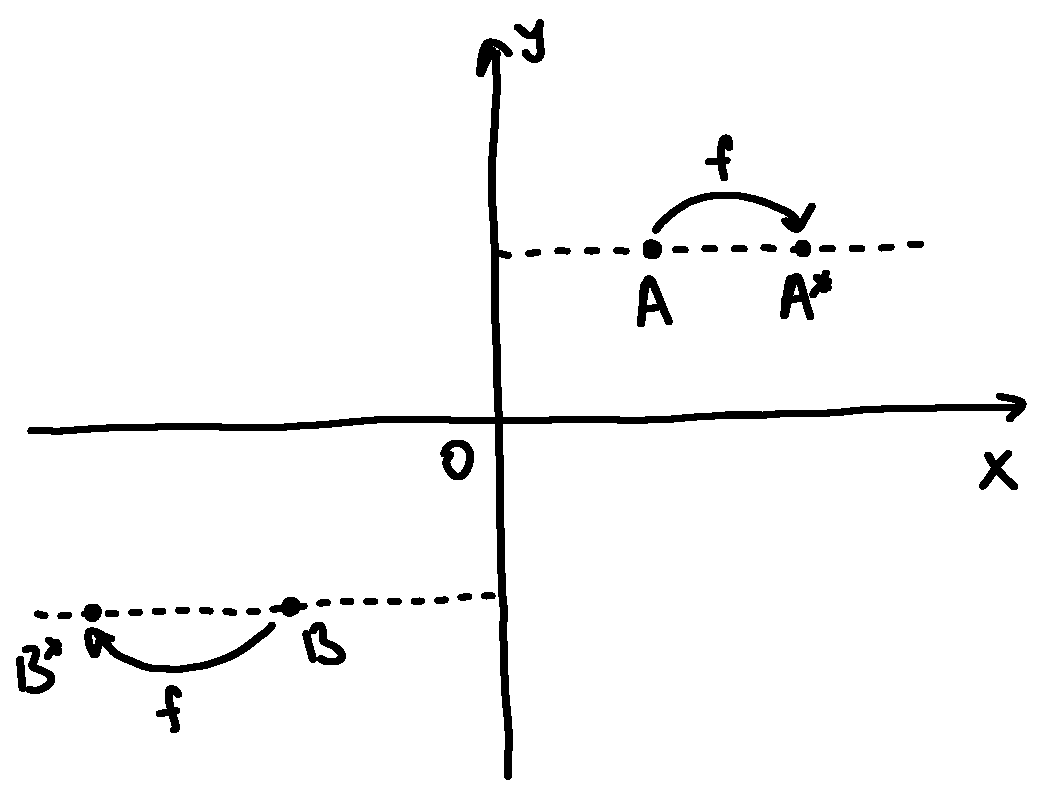
\includegraphics[width=0.6\columnwidth]{linear-example}
      
      \caption{Преобразование растяжения вдоль оси $OX$ в $2$ раза (\emph{сжатия к прямой} $x \hm= 0$ с коэффициентом $2$).}
      \label{fig:linear-example}
    \end{figure}
    
    Что происходит в результате действия~$f$?
    Если взять точку $A(x_a, y_a)$, $x_a \hm> 0$, то она перейдёт в точку $A^*$, расположенную ``правее'', на том же уровне от оси $X$, и в два раза дальше от оси $Y$.
    Если же взять точку $B(x_b, y_b)$, $x_b \hm< 0$, то она пойдёт ``влево'' до точки $B^*$, также удалённой от оси $Y$ на в два раза большее расстояние.
    То есть суть преобразования $f$ в том, что все точки плоскости ``расходятся'' от оси $Y$.
    
    Такое преобразование называют \emph{сжатием к прямой с коэффициентом $k$}.
    В рассмотренном примере~---~сжатие к прямой, являющейся осью $OY$, с коэффициентом $2$.
    (Когда ``коэффициент сжатия'' больше нуля, то можно преобразование называть \emph{растяжением относительно прямой с коэффициентом $k$}.)
  \end{example}
  
  \begin{example}
    Линейным будет, например, преобразование поворота плоскости на угол $\phi$ вокруг начала координат.
    
    \begin{figure}
      \centering
      
      \includegraphics[width=0.6\columnwidth]{rotate-around-zero-inv}
      
      \caption{Поворот плоскости вокруг начала координат на угол~$\phi$.}
      \label{fig:rotate-around-zero-inv}
    \end{figure}
    
    Получим его формулу.
    При повороте плоскости точка $A(x, y)$, отличная от начала координат, перейдёт в точку $A^*(x^*, y^*)$ (см. рисунок~\ref{fig:rotate-around-zero-inv}).
    Если ввести обозначения: $a$ для длины радиуса-вектора точки $A$ и $\alpha$ для угла между радиусом-вектором точки $A$ и положительным направлением оси $X$~---~то можно записать:
    \[
      \left\{
        \begin{aligned}
          &x = a \cos \alpha\\
          &y = a \sin \alpha
        \end{aligned}
      \right.
    \]
    
    С другой стороны, расстояние от образа $A^*$ до начала координат не изменилось, поэтому также можем записать:
    \[
      \left\{
        \begin{aligned}
          &x^* = a \cos(\alpha + \phi) = \underbrace{a \cos\alpha}_{x} \cos\phi - \underbrace{a \sin\alpha}_{y} \sin\phi\\
          &y^* = a \sin(\alpha + \phi) = \underbrace{a \sin\alpha}_{y} \cos\phi + \underbrace{a \cos\alpha}_{x} \sin\phi
        \end{aligned}
      \right.
    \]
    
    Итого, формула для преобразования поворота вокруг начала координат:
    \begin{equation}\label{eq:rotate-around-zero}
      \boxed{
        \left\{
          \begin{aligned}
            &x^* = x \cos\phi - y \sin\phi\\
            &y^* = x \sin\phi + y \cos\phi
          \end{aligned}
        \right.
      }
    \end{equation}
  \end{example}
  
  Точка~$M$ называется \emph{неподвижной} точкой преобразования~$f$, если её образ и есть она сама: $M \hm= f(M)$.
  У преобразования поворота вокруг начала координат~(\ref{eq:rotate-around-zero}), очевидно, есть единственная неподвижная точка~---~начало координат.
  У другого рассмотренного в качестве примера линейного преобразования~(\ref{eq:linear-example}) начало координат тоже неподвижно...
  Более того, неподвижна целая ось $OY$!
  Множество точек $\mathcal M$ называется \emph{неподвижным} относительно преобразования~$f$, если все его точки неподвижны: $f(M) \hm= M$, $\forall M \hm\in \mathcal M$.
  
  Неподвижное множество точек~---~когда все остаются ``не том же месте''.
  Если мы ``ослабим'' условие, то придём к более общему понятию.
  Множество точек~$\mathcal M$ называется \emph{инвариантным}, если образ любой точки $M$ множества лежит в том же множестве: $f(M) \hm\in \mathcal M$, $\forall M \hm\in \mathcal M$.
  У преобразования поворота~(\ref{eq:rotate-around-zero}) нет других инвариантных множеств, кроме множества из одной точки~--~начала координат, и множества, состоящего из всех точек плоскости.
  У преобразования же из примера~(\ref{eq:linear-example}) есть ``более интересные'' инвариантные множества.
  Например, неподвижная ось~$OY$.
  Но, помимо этого, инвариантной будет любая прямая, параллельная оси $OX$~(\ref{fig:linear-example-inv}).
  
  \begin{figure}
      \centering
      
      \includegraphics[width=0.6\columnwidth]{linear-example-inv}
      
      \caption{Инвариантные множества относительно преобразования сжатия к прямой $x \hm= 0$ с коэффициентом $k \hm= 0$.}
      \label{fig:linear-example-inv}
    \end{figure}
  
  Линейное преобразование плоскости $f$ порождает следующее преобразование векторов:
  \[
    \vv{AB} \overset{f}{\mapsto} \vv{f(A)f(B)}
  \]
  Преобразование векторов можно обозначать той же буквой, что и преобразование координат (по контексту должно быть понятно, о каком преобразовании идёт речь).
  Координатная запись преобразования, которое переводит вектор $\bds v \hm= (\alpha, \beta)$ в вектор $\bds v^\star \hm= (\alpha^\star, \beta^\star)$:
  \begin{equation}
    \left\{
      \begin{aligned}
          &\alpha^\star = a_1 \alpha + b_1 \beta\\
          &\beta^\star = a_2 \alpha + b_2 \beta
      \end{aligned}
    \right.
  \end{equation}
  
  Откуда можно заметить, что преобразование векторов $f$ \emph{линейно} в том смысле, что сохраняет линейные операции между векторами:
  \[
    \left\{
      \begin{aligned}
        &f(\bds v + \bds u) = f(\bds v) + f(\bds u)\\
        &f(\lambda \bds v) = \lambda f(\bds v),\quad \lambda \in \RR
      \end{aligned}
    \right.
  \]
  
  В качестве линейного преобразования можно привести, например, преобразование поворота~(\ref{eq:rotate-around-zero}).
  И то преобразование, переводящее плоскость в одну точку (например в ноль)
  \[
    \left\{
      \begin{aligned}
        &x^\star = 0\\
        &y^\star = 0
      \end{aligned}
    \right.
  \]
  тоже будет линейным, но, очевидно, не будет ни инъективным, ни сюръективным...
  
  
  \subsection{Про аффинные преобразования}
  
  \begin{definition}
    \emph{Аффинным} называется взаимно однозначное (биективное) преобразование плоскости.
  \end{definition}
  
  % TODO: про то, что наличие обратного сильнее биективности
  
  Поворот будет аффинным преобразованием, а отображение в одну точку~---~уже не будет аффинным.
  \emph{Критерием аффинности} преобразования~---~чтобы всегда (при любых $x^*$, $y^*$) существовало единственно решение системы~(\ref{eq:linear})~---~является отличие от нуля определителя системы:
  \[
    \boxed{
      \begin{vmatrix} a_1 & b_1\\ a_2 & b_2\end{vmatrix} \not= 0
    }
  \]
  
  Можно заметить, что
  
  \begin{proposition}
    Аффинное преобразование определяется образами трёх точек, не лежащих на одной прямой.
  \end{proposition}
  
  \begin{proof}
    Это несложно понять из такого рассуждения.
    
    Пусть три точки: $O$, $A$ и $B$~---~не лежат на одной прямой.
    Тогда можно выбрать систему координат с началом в $O$ и базисными векторами $\vv{OA}$ и $\vv{OB}$.
    Положение любой точки $M$ плоскости определяется её радиусом-вектором (положением относительно точки $O$):
    \[
      \vv{OM} = \alpha \vv{OA} + \beta \vv{OB}
    \]
    
    Пусть есть аффинное преобразование~$f$.
    Оно переводит точки $O$, $A$ и $B$ в соответственно точки $O^*$, $A^*$ и $B^*$.
    Они также не лежат на одной прямой (почему?).
    То есть $O^*$ и $\vv{O^*A^*}$, $\vv{O^*B^*}$ тоже можно бы было выбрать в качестве системы координат.
    При этом положение образа~$M^*$ любой точки~$M$ расположено относительно~$O^*$ так же, как сама точка~$M$ расположена относительно~$O$:
    \[
      \vv{O^*M^*} = \alpha \vv{O^*A^*} + \beta \vv{O^*B^*}
    \]
    
    Таким образом, устанавливается взаимно однозначное соответствие между точками-прообразами и точками-образами.
    Причём линейное (сохраняются линейные операции между векторами).
    Это и означает единственность аффинного преобразования.
    Другими словами, коэффициенты в формулах преобразования определены однозначно (какие они в итоге будут, коэффициенты?).
    То есть~$f$ однозначно определяется образами $O$, $A$ и~$B$.
  \end{proof}
  
  
  \subsubsection{Действие на прямую и кривую второго порядка}
  
  До сих пор мы обращали внимание только на точки и векторы.
  На то, что происходит с ними в результате действия аффинного преобразования.
  Посмотрим теперь, как меняются ``более сложные'' объекты.
  
  \begin{proposition}[Прямая]
    Под действием аффинного преобразования $f$ прямая переходит в прямую.
  \end{proposition}
  
  \begin{proof}
    Чем можно задать прямую?
    Например, начальной точкой~$M_0$ и направляющим вектором~$\bds a$.
    Каждая точка~$M$ прямой $l$ (радиус-вектор каждой точки прямой) получается из начальной сдвигом вдоль направляющего на некоторый ``шаг''~$t$.
    Мы можем посчитать образ начальной точки~$f(M_0)$ и образ направляющего вектора прямой~$f(\bds a)$.
    Тогда, очевидно, образ любой другой точки прямой~$f(M)$ отстоит от образа начальной на такой же ``шаг''~$t$, но уже вдоль вектора~--~образа направляющего~$f(\bds a)$.
    Получается, образы всех точек~$l$ лежат на прямой~$l^*$, определяемой $f(M_0)$ и $f(\bds a)$.
    
    Если это же расписать ``более строго'', то получится:
    \[
      \vv{OM} = \vv{OM_0} + \bds a t
    \]
    
    С одной стороны:
    \[
      f(\vv{OM}) = \vv{O^*M^*} = \vv{O^*O} + \vv{OM^*}
    \]
    
    С другой:
    \[
      f(\vv{OM}) = f(\vv{OM_0} + \bds a t) = \vv{O^*M_0^*} + f(\bds a) t
    \]
    
    Поэтому для радиуса-вектора точки-образа получаем:
    \[
      \vv{OM^*} = f(\vv{OM}) - \vv{O^*O} = \bigl(\vv{OO^*} + \vv{O^*M_0^*}\bigr) + f(\bds a) t
    \]
    
    Обратно, можно убедиться, что любая точка прямой~$l^*$ обязательно является образом некоторой точки прямой~$l$.
    Поэтому образ прямой~$l$ есть~$l^*$.
  \end{proof}
  
  
  \begin{proposition}[Отрезок]
    Аффинное преобразование $f$ переводит в отрезок.
  \end{proposition}
  
  \begin{proof}
    Основные рассуждения~---~такие же, как в случае с прямой.
    Только параметр~$t$ отрезка-прообраза теперь варьируется не как $t \hm\in \RR$, а как $t \hm\in [t_1, t_2]$.
  \end{proof}
  
  
  \begin{proposition}[Параллельные прямые]
    Аффинное преобразование $f$ переводит параллельные прямые в параллельные прямые.
  \end{proposition}
  
  \begin{proof}
    Если допустить, что образы не параллельны, то они пересекаются~---~значит, есть общая точка, у которой два различных прообраза (по одному на каждой из исходных параллельных прямых).
    Но это~---~противоречие с взаимной однозначностью преобразования~$f$.
  \end{proof}
  
  
  \begin{proposition}[Кривая второго порядка]
    Аффинное преобразование $f$ переводит кривую второго порядка в кривую второго порядка.
  \end{proposition}
  
  \begin{proof}
    Понять, почему это так, можно из следующего наблюдения.
    Пусть исходная кривая (эллипс/гипербола/...) задаётся уравнением второй степени вида
    \[
      F(x, y) = 0
    \]
    
    В результате аффинного преобразования каждая точка~$(x, y)$ кривой переходит в точку~$(x^*, y^*)$.
    Чтобы получить уравнение образа кривой, можно из системы, задающей аффинное преобразование, выразить, наоборот, исходные координаты $x$ и $y$ через $x^*$ и $y^*$.
    (Получается ``обратная замена'', которая тоже есть аффинное преобразование.)
    И подставить в уравнение:
    \[
      F\bigl(x(x^*, y^*), y(x^*, y^*)\bigr) = 0
    \]
    
    После ``раскрытия скобок'' и упрощений получаем уравнение образа кривой:
    \[
      F^*(x^*, y^*) = 0
    \]
    
    Степень $F^*$ не могла повыситься, потому что аффинная замена~---~линейная.
    Но она также не могла понизиться.
    Потому что, если допустить обратное, получится, что обратный переход, от образа к прообразу, повышает степень уравнения, чего быть не может (так как и само преобразование, и обратное к нему~---~аффинные).
    
    Таким образом, уравнение с~$F^*$ тоже второй степени.
  \end{proof}
  
  
  \begin{proposition}[Класс кривой второго порядка]
    Аффинное преобразование $f$ сохраняет класс кривой второго порядка (эллипс/гипербола/... переходит в соответственно эллипс/гиперболу/...).
  \end{proposition}
  
  \begin{example}
    Не будем пытаться доказать это ``строго''.
    Вместо этого рассмотрим пример.
    
    Пусть ``некоторое'' аффинное преобразование~$f$ задаётся в некоторой прямоугольной системе координат следующей системой уравнений:
    \[
      f\colon \left\{
        \begin{aligned}
          &x^* = x \sqrt{2} - y \sqrt{2} + 1\\
          &y^* = \frac{3}{\sqrt{2}} x + \frac{3}{\sqrt{2}} y - 17.5
        \end{aligned}
      \right.
    \]
    
    ``Что происходит'' в результате~$f$?
    Систему можно переписать следующим образом:
    \[
      f\colon \left\{
        \begin{aligned}
          &x^* = \textcolor{my-red}{2} \textcolor{my-red}{\cdot} \left(\textcolor{my-blue}{\frac{1}{\sqrt{2}}} x \textcolor{my-blue}{-} \textcolor{my-blue}{\frac{1}{\sqrt{2}}} y\right) \textcolor{my-cyan}{+} \textcolor{my-cyan}{1}\\
          &y^* = \textcolor{my-red}{3} \textcolor{my-red}{\cdot} \left(\textcolor{my-blue}{\frac{1}{\sqrt{2}}} x \textcolor{my-blue}{+} \textcolor{my-blue}{\frac{1}{\sqrt{2}}} y\right) \textcolor{my-cyan}{-} \textcolor{my-cyan}{17.5}
        \end{aligned}
      \right.
    \]
    
    То есть преобразование~$f$ есть как бы последовательное применение нескольких преобразований, \emph{композиция}: поворот~$\textcolor{my-blue}{g_1}$ на $45\degree$ вокруг начала координат, растяжение~$\textcolor{my-red}{h_1}$ вдоль одной оси в $2$ раза, растяжение~$\textcolor{my-red}{h_2}$ вдоль другой оси в $3$ раза и параллельный перенос~$\textcolor{my-cyan}{g_2}$ на вектор $(1, -17.5)$:
    \[
      f = \textcolor{my-cyan}{g_2} \textcolor{my-red}{h_2} \textcolor{my-red}{h_1} \textcolor{my-blue}{g_1}
      \Leftrightarrow f(x) = \textcolor{my-cyan}{g_2}\biggl(
        \textcolor{my-red}{h_2}\Bigl(
          \textcolor{my-red}{h_1}\bigl(
            \textcolor{my-blue}{g_1}(x)
          \bigr)
        \Bigr)
      \biggr)
      \quad \forall x \mbox{~---~точки плоскости}
    \]
    
    Но тогда не сложно заметить, что, например, эллипс останется эллипсом.
    И то же самое и для гиперболы и параболы: класс кривой сохраняется.
    
    Да, произвольное аффинное преобразование может не получиться \emph{сразу} представить как композицию.
    Но далее мы увидим, что всё равно любое аффинное преобразование в итоге сводится к параллельному переносу, повороту (возможно, и отражению) и растяжениям.
  \end{example}
  
  
  \begin{proposition}[Пара кривых одного класса]
    Помимо того, что аффинное преобразование~$f$ сохраняет класс кривой второго порядка, оказывается, что для любых двух кривых второго порядка одного класса существует аффинное преобразование, которое переводит одну кривую в другую.
  \end{proposition}
  
  \begin{example}
    Опять, ``отложим в сторону попытки'' это в каком-то смысле строго обосновать, и лучше посмотрим на пример.
    Пусть есть два эллипса~(\ref{fig:from-ellipse-to-ellipse}).
    Как нам из ``одного'' получить ``другой''?
    Очевидно, что можно начать, например, с поворота: повернём первый эллипс так, чтобы его оси стали параллельны осям второго эллипса.
    Далее, можно совместить центры эллипсов с помощью параллельного переноса.
    Теперь остаётся только растянуть первый эллипс (уже повёрнутый и перенесённый) вдоль осей до совпадения со вторым.
    
    \begin{figure}
      \centering
      
      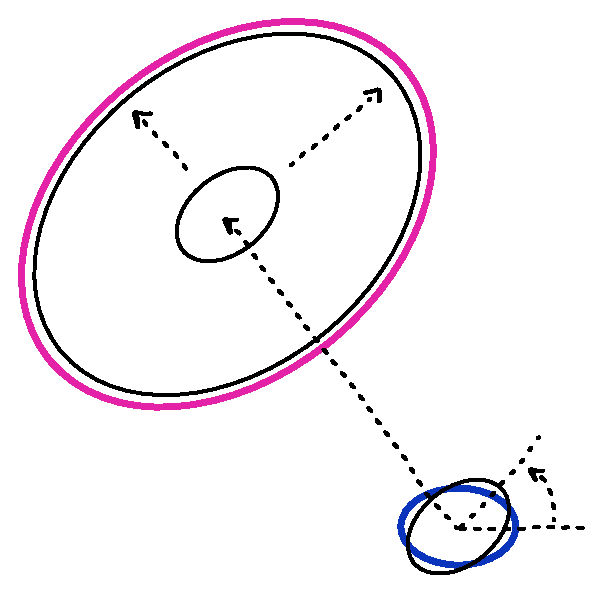
\includegraphics[width=0.5\columnwidth]{from-ellipse-to-ellipse}
      
      \caption{Как из ``одного'' эллипса получить ``другой'' с помощью аффинного преобразования: поворот, перенос, растяжение.}
      \label{fig:from-ellipse-to-ellipse}
    \end{figure}
  \end{example}
  
  
  
  \subsubsection{Изменение площади и длины}
  
  Точки переходят в точки, векторы в векторы, кривые в кривые.
  Но... какие ``изменения'' при этом происходят?
  Например, можно задаться вопросом о том, как меняется \emph{площадь} фигуры в результате аффинного преобразования.
  
  В случае с эллипсом вполне можем это выяснить: эллипс переходит в эллипс, а его площадь определяется величинами большой и малой полуосей.
  Таким образом, зная длины осей, узнаем площадь.
  А оси несложно достать из уравнения эллипса...
  Но как быть с ``более сложными'' фигурами?
  
  Можно смотреть на площадь произвольной фигуры как на сумму ``элементарных'' площадей.
  Например, можно разбить фигуру на ``маленькие квадратики''.
  Если, например, окажется, что площадь одного такого квадратика меняется в $k$ раз, то и площадь всей фигуры, очевидно, изменится в то же самое число раз $k$ (при этом понимаем, что под действием аффинного преобразования квадратик переходит в параллелограмм).
  Таким образом, сначала стоит понять, что происходит с ``квадратиком''.
  
  Пусть аффинное преобразование задано формулами:
  \begin{equation}\label{eq:affine-for-square-and-length}
    f\colon \left\{
      \begin{aligned}
        &x^* = a_1 x + b_1 y + c_1\\
        &y^* = a_2 x + b_2 y + c_2
      \end{aligned}
    \right.
  \end{equation}
  
  И рассмотрим квадрат, построенный на базисных векторах $\bds e_1$ и $\bds e_2$ (система координат, как и обычно во всех номерах про аффинные, декартова прямоугольная).
  Его площадь $S \hm= S(\bds e_1, \bds e_2) \hm= 1$.
  Далее, под действием $f$ произойдёт следующее: вектор $\bds e_1$ перейдёт в вектор $f(\bds e_1)$, вектор $\bds e_2$ перейдёт в вектор $f(\bds e_2)$~---~которые также не коллинеарны~---~а исходный параллелограмм, построенный на $\bds e_1, \bds e_2$ станет параллелограммом, который построен на $f(\bds e_1), f(\bds e_2)$.
  Его площадь $S'$ можно посчитать с помощью векторного произведения (перед этим вводим третью ось $OZ$ так, чтобы система координат $XYZ$ была правой прямоугольной):
  \[
    S' = S'\bigl(f(\bds e_1), f(\bds e_2)\bigr) = |\bds c|,\quad \bds c = [f(\bds e_1) \times f(\bds e_2)] = \begin{vmatrix}
      a_1 & a_2\\
      b_1 & b_2
    \end{vmatrix} = \begin{vmatrix}
      a_1 & b_1\\
      b_2 & b_2
    \end{vmatrix}
  \]
  
  Где воспользовались тем, что, например, $f(\bds e_1) \hm= (1 \hm\cdot a_1 \hm+ 0 \hm\cdot b_1, 1 \hm\cdot a_2 \hm+ 0 \hm\cdot b_2) \hm= (a_1, a_2)$.
  И в последнем переходе, где вычисляется $\bds c$, использовали то, что определитель матрицы не изменится при указанной перестановке элементов (\emph{транспонирование}).
  
  Таким образом, отношение площадей образа и самого квадратика:
  \[
    S'_{\pm}/S_{\pm} = \begin{vmatrix}
      a_1 & b_1\\
      b_2 & b_2
    \end{vmatrix}
  \]
  
  Причём выражение, стоящее справа, больше нуля, если ориентация пары $\bigl(f(\bds e_1), f(\bds e_2)\bigr)$ такая же, как и пары $(\bds e_1, \bds e_2)$.
  И меньше нуля~---~если ориентация другая (поворот от первого вектора ко второму происходит, например, по часовой стрелке, а до этого было ``против'').
  Поэтому в левой части формулы используются обозначения площадей с индексом $\pm$~---~площадь со знаком.
  
  Площади ``сложных фигур'' относятся подобным же образом: модуль определителя матрицы преобразования говорит о том, во сколько раз изменяется площадь.
  А знак определителя~---~о том, меняется или нет ориентация пары векторов, которые есть образы базисных.
  
  
  \bigskip
  
  С площадью разобрались.
  А что происходит с длиной?
  Лучше даже зададимся вопросом: может ли аффинное преобразование сохранять длины? при каких условиях?
  
  Рассмотрим произвольный вектор $\bds v \hm= (\alpha, \beta)$.
  Под действием аффинного преобразования~(\ref{eq:affine-for-square-and-length}) он перейдёт в вектор
  \[
    \bds v^* = (a_1 \alpha + b_1 \beta, a_2 \alpha + b_2 \beta)_{\bds e_1, \bds e_2}
             = (\alpha, \beta)_{f(\bds e_1), f(\bds e_2)}
  \]
  
  Где в последнем переходе воспользовались тем, что вектор $\bds v^*$ имеет в базисе $\bigl(f(\bds e_1), f(\bds e_2)\bigr)$ такие же координаты, как вектор $\bds v$ в базисе $(\bds e_1, \bds e_2)$:
  \[
    \bds v^* = f(\bds v) = f(\alpha \bds e_1 + \beta \bds e_2) = \alpha f(\bds e_1) + \beta f(\bds e_2)
  \]
  
  Квадрат длины исходного вектора\footnote{Формула записана так, чтобы быть верной и в случае общего базиса, не только ортонормированного.}:
  \[
    |\bds v|^2 = (\bds v, \bds v) = \alpha^2 (\bds e_1, \bds e_1) + 2 \alpha \beta (\bds e_1, \bds e_2) + \beta^2 (\bds e_2, \bds e_2)
  \]
  
  Квадрат длины вектора-образа:
  \[
    |\bds v^*|^2 = (\bds v^*, \bds v^*) = \alpha^2 \bigl(f(\bds e_1), f(\bds e_1)\bigr) + 2 \alpha \beta \bigl(f(\bds e_1), f(\bds e_2)\bigr) + \beta^2 \bigl(f(\bds e_2), f(\bds e_2)\bigr)
  \]
  
  Таким образом, сохранение длины $|\bds v^*| \hm= |\bds v|$ для произвольного вектора $\bds v$ равносильно выполнению условий:
  \[
    \boxed{
      \left\{
        \begin{aligned}
          &(\textcolor{my-red}{\bds e_1}, \textcolor{my-red}{\bds e_1}) = \bigl(f(\textcolor{my-red}{\bds e_1}), f(\textcolor{my-red}{\bds e_1})\bigr)\\
          &(\textcolor{my-blue}{\bds e_2}, \textcolor{my-blue}{\bds e_2}) = \bigl(f(\textcolor{my-blue}{\bds e_2}), f(\textcolor{my-blue}{\bds e_2})\bigr)\\
          &(\textcolor{my-red}{\bds e_1}, \textcolor{my-blue}{\bds e_2}) = \bigl(f(\textcolor{my-red}{\bds e_1}), f(\textcolor{my-blue}{\bds e_2})\bigr)
        \end{aligned}
      \right.
    }
  \]
  
  Преобразование, сохраняющее длины, называется \emph{ортогональным}.
  Итого, преобразование ортогонально, если и только если оно сохраняет длины базисных векторов и угол между ними.
  
  Несложно видеть, что ортогональным может быть только поворот (или отражение) и параллельный перенос.
  Или их композиция.
  Отсюда получаем ещё одно небезынтересное наблюдение.
  Матрица ортогонального преобразования~---~это обязательно матрица поворота (``с синусами и косинусами'').
  
  
  \subsubsection{Аффинное как композиция}
  
  Снова обратимся к примеру.
  
  \begin{example}
    Рассмотрим пару эллипсов.
    Существует аффинное преобразование, которое переводит один в другой.
    При этом аффинное преобразование однозначно определяется образами трёх точек, не лежащих на одной прямой.
    Потребуем, чтобы вершины эллипса $A$ и $B$ переходили в вершины (обозначим их потому $A^*$ и $B^*$), и центр $O$~---~в центр $O^*$.
    Этим однозначно определяется аффинное преобразование, причём такое, которое переводит первый эллипс во второй.
    
    Что интересного можно заметить?
    Векторы, задающие направления осей исходного эллипса, были перпендикулярны:
    \[
      \vv{OA} \perp \vv{OB}
    \]
    
    Но и их образы~---~тоже перпендикулярны!
    \[
      \vv{O^*A^*} \perp \vv{O^*B^*}
    \]
    
    Более того, перпендикулярными остались целых два \emph{направления}, задаваемые векторами $\vv{OA}$ и $\vv{OB}$.
    Такие направления называются \emph{главными}, или \emph{сингулярными} направлениями аффинного преобразования.
  \end{example}
  
  Далее, уже на конкретном примере (при решении задач), мы убедимся в том, что \emph{у любого аффинного преобразования есть пара сингулярных направлений}.
  Также, в той же задаче, которая будет решена далее\footnote{Забавно, сказав, что такая вот задача будет решена в будущем, мы фактически определили \href{https://docs.python.org/3/library/asyncio-future.html\#asyncio.Future}{асинхронную задачу}: ``что-то, что ещё не готово, но будет готово в будущем''. ``По-настоящему асинхронной'' она бы была, если бы, например, в процессе оформления конспекта далее, вместо того, чтоб прерваться на ``попить чай'', автор конспекта бы ``переключался'', перепрыгивал вперёд сразу на оформление куска с решением указанной задачи. (То есть чередование: то изложение материала в конспекте далее, то решение сразу указанной задачи про разложение аффинного, скачки туда-сюда.) Anyway...} мы проверим, что
  
  \begin{proposition}
    Любое аффинное преобразование~$f$ может быть представлено как композиция
    \[
      f = h_2 h_1 g
    \]
    
    Где $g$~---~ортогональное преобразование, а $h_1$ и $h_2$~---~сжатия к двум взаимно перпендикулярным прямым.
  \end{proposition}
  
  Причём эти $h_1$ и $h_2$~---~это будут сжатия к прямым, которые параллельны как раз сингулярным направлениям.
  
  
  \section{Задачи}
  
  Начнём с небольшой задачи на свойства ``абстрактного'' отображения.
  
  
  \subsection{\# 12.1(2, 4)}
  
  Для отображения $f\colon \mathcal X \to \mathcal Y$ доказать, что
  
  \begin{enumerate}
    \setcounter{enumi}{1}
    
    \item $f(A_1 \cup A_2) = f(A_1) \cup f(A_2)$
    
    \setcounter{enumi}{3}
    
    \item $f(A_1 \cap A_2) \subseteq f(A_1) \cap f(A_2)$
  \end{enumerate}
  
  \begin{solution}
    Начнём с первого пункта.
    Чтобы доказать требуемое, достаточно показать, что произвольная точка из $f(A_1 \cup A_2)$ лежит также и в $f(A_1) \cup f(A_2)$ и наоборот, что произвольная точка из $f(A_1) \cup f(A_2)$ лежит также и в $f(A_1 \cup A_2)$.
    
    Пусть $y \hm\in f(A_1 \cup A_2)$.
    Это значит, что $\exists x \hm\in A_1 \hm\cup A_2\colon f(x) \hm= y$.
    Если $x \hm\in A_1$, то $f(x) \hm\in f(A_1)$, если же $x \hm\in A_2$, то $f(x) \hm\in f(A_2)$.
    В любом случае $f(x) \hm\in f(A_1) \hm\cup f(A_2)$.
    
    Пусть теперь $y \hm\in f(A_1) \hm\cup f(A_2)$.
    Это значит, что $\exists x \hm\in A_1\colon f(x) \hm= y$ или $\exists x \hm\in A_2\colon f(x) \hm= y$.
    Но это можно переписать как $\exists x \hm\in A_1 \hm\cup A_2\colon f(x) \hm= y$, а это и значит, что $f(x) \hm\in f(A_1 \cup A_2)$.
    
    \bigskip
    
    Теперь докажем второй пункт.
    Пусть $y \hm\in f(A_1 \cap A_2)$.
    Это значит, что $\exists x \hm\in A_1 \hm\cap A_2\colon f(x) \hm= y$.
    Из того, что $x \hm\in A_1$, следует, что $f(x) \hm\in f(A_1)$.
    Аналогично, $x \hm\in A_2 \hm\Rightarrow f(x) \hm\in f(A_2)$.
    В итоге $f(x) \hm\in f(A_1) \hm\cap f(A_2)$.
    
    Покажем, что второе включение не выполняется, то есть что может $\exists y \hm\in f(A_1) \hm\cap f(A_2)$, такой что $y \hm{\not\in} f(A_1 \cap A_2)$.

    \begin{figure}
      \centering
      
      \includegraphics[width=0.8\columnwidth]{cap-not-cap}
      
      \caption{$A_1, A_2$ и $f$, такие что $f(A_1) \hm\cap f(A_2) \hm{\not=} \noth$, но $A_1 \hm\cap A_2 \hm= \noth$.}
      \label{fig:cap-not-cap}
    \end{figure}

    Выберем $A_1$ и $A_2$ так, чтобы $f(A_1) \hm\cap f(A_2) \hm{\not=} \noth$ (отображение $f$, хоть и ``дано в условии'', произвольное, и его тоже можно подбирать) и $A_1 \hm\cap A_2 \hm= \noth$ (\ref{fig:cap-not-cap}).
    И получаем, что $\bigl(f(A_1) \hm\cap f(A_2)\bigr) \hm\cap f(A_1 \cap A_2) \hm= \noth$.
  \end{solution}
  
  
  \subsection{\# 12.28(1)}
  
  Доказать, что если $A$ и $B$~---~две различные неподвижные точки аффинного преобразования $f$, то и все точки прямой $AB$ неподвижны.
  
  \begin{solution}
    Очевидно, прямая $AB$ перейдёт в прямую $A^*B^* \hm= AB$, то есть прямая инвариантна.
    Тогда проверим, что она, кроме того, ещё и неподвижна.
    
    Выберем в качестве начальной точки на прямой $AB$ точку $A$.
    В качестве направляющего вектора~---~вектор $\vv{AB} \hm\equiv \bds a$.
    (Итого, выбрали \emph{локальную систему координат} на прямой.)
    Для произвольной точки $M$ прямой $AB$ верно, что
    \[
      \vv{OM} = \vv{OA} + \vv{AB} \cdot t
    \]
    
    Где как $O$ обозначили начало некоторой системы координат на плоскости\footnote{Могли бы в качестве $O$ выбрать саму точку $A$. Было бы проще. Но ``в демонстрационных целях'' намеренно усложним задачу, чтоб выкладки были ``более общими''...}.
    
    Образ точки $M$:
    \[
      \vv{OM^*} = \vv{OO^*} + \vv{O^*M^*} = \vv{OO^*} + \vv{O^*A^*} + f(\vv{AB}) t
        = \underbrace{\vv{OO^*} + \vv{O^*A}}_{\vv{OA}} + \vv{AB} \cdot t
        = \vv{OM}
    \]
    
    Совпадает с $M$.
  \end{solution}


  \subsection{\# 9.13(1)}
  
  Определить тип кривой второго порядка
  \[
    (3x - 4y)^2 - 5(x + 2y - 1)^2 = 1
  \]
  
  \begin{solution}
    Сделаем напрашивающуюся замену:
    \[
      \left\{
        \begin{aligned}
          &x^\star = 3x - 4y\\
          &y^\star = x + 2y - 1
        \end{aligned}
      \right.
    \]
    
    Преобразование, очевидно, линейное.
    Определитель системы отличен от нуля, поэтому преобразование взаимно однозначное.
    И в итоге~---~аффинное.
    А кривая
    \[
      (x^\star)^2 - 5(y^\star)^2 = 1
    \]
    очевидно, является гиперболой.
    Так как при аффинном преобразовании тип кривой второго порядка сохраняется, то и исходная система описывает гиперболу.
    (Гиперболы разные, уравнение со ``звёздочными'' координатами описывает \emph{другую} гиперболу, но класс кривой один.)
  \end{solution}
  
  
  \subsection{\# 12.48(1)}
  
  Дано аффинное преобразование
  \[
    \left\{
      \begin{aligned}
        &x^* = 2x + 3y\\
        &y^* = 3x + 5y
      \end{aligned}
    \right.
  \]
  
  Надо составить уравнение образа кривой $x^2 \hm+ y^2 \hm= 1$.
  
  \begin{solution}
    Перепишем уравнение исходной кривой в виде:
    \[
      \underbrace{x^2 + y^2 - 1}_{F(x, y)} = 0
    \]
    
    Уравнение образа кривой~---~соотношение между координатами точек, такое что точки образа и только они удовлетворяют этому соотношению.
    Аффинное преобразование взаимно однозначно~---~значит, можно выразить исходные координаты $x, y$ через $x^*, y^*$:
    \[
      \left\{
        \begin{aligned}
          &x = x(x^*, y^*) = \ldots = 5x^* - 3y^*\\
          &y = y(x^*, y^*) = \ldots = -3x^* + 2y^*
        \end{aligned}
      \right.
    \]
    
    Таким образом, уравнение исходной кривой ``переходит'' в уравнение образа кривой:
    \begin{equation*}
    \begin{split}
      F(x, y) = 0 &\Leftrightarrow x^2 + y^2 - 1 = 0\\
                  &\Leftrightarrow x^2(x^*, y^*) + y^2(x^*, y^*) - 1 = 0\\
                  &\Leftrightarrow (5x^* - 3y^*)^2 + (-3x^* + 2y^*)^2 - 1 = 0\\
                  &\Leftrightarrow \underbrace{{34x^*}^2 - 42x^*y^* + {13y^*}^2 - 1}_{F^*(x^*, y^*)} = 0\\
                  &\Leftrightarrow F^*(x^*, y^*) = 0
    \end{split}
    \end{equation*}
  \end{solution}
  
  
  \subsection{\# 12.53(6, 9)}
  
  Вывести формулы, задающие данные преобразования плоскости:
  \begin{enumerate}
    \setcounter{enumi}{5}
    
    \item Симметрия относительно прямой $l\colon 3x + 4y - 1 = 0$
    
    \setcounter{enumi}{7}
    
    \item Сжатие к прямой $m\colon 2x - y + 5 = 0$ с коэффициентом $k \hm= 2$
  \end{enumerate}
  
  \begin{solution}
    \begin{figure}
      \centering
      
      \includegraphics[width=0.5\columnwidth]{simmetria-linea}
      
      \caption{Преобразование симметрии относительно прямой.}
      \label{fig:simmetria-linea}
    \end{figure}
    
    Чтобы получить уравнения, задающие симметрию относительно прямой, рассмотрим произвольную точку плоскости $M(x, y)$ (\ref{fig:simmetria-linea}).
    Образ этой точки~---~точка $M^\star(x^\star, y^\star)$.
    Введём дополнительно точку $M_\perp$~---~ортогональную проекцию точки $M$ на прямую $l$.
    Симметрия относительно прямой~---~такое преобразование, что $\vv{M^\star M} \hm= 2 \vv{M_\perp M}$.
    Выпишем все получившиеся условия, чтобы потом переписать их через координаты точек
    \[
      \left\{
        \begin{aligned}
          &\vv{M_\perp M} \perp l\\
          &M_\perp \in l\\
          &\vv{M^\star M} = 2 \vv{M_\perp M}
        \end{aligned}
      \right.
    \]
    
    Из первых двух уравнений можно найти координаты точки $M_\perp(x_1, y_1)$:
    \[
      \left\{
        \begin{aligned}
          &(x_1 - x_0) \cdot (-4) + (y_1 - y_0) \cdot 3 = 0\\
          &3x_1 + 4y_1 - 1 = 0
        \end{aligned}
      \right.
      \Rightarrow \ldots
      \Rightarrow \left\{
        \begin{aligned}
          &x_1 = \frac{3 + 16x_0 - 12y_0}{25}\\
          &y_1 = \frac{4 - 12x_0 + 9y_0}{25}
        \end{aligned}
      \right.
    \]
    
    И координаты точки-образа можно найти как
    \[
      \left\{
        \begin{aligned}
          &x^\star = x_0 + 2 \cdot (x_1 - x_0)\\
          &y^\star = y_0 + 2 \cdot (y_1 - y_0)
        \end{aligned}
      \right.
    \]
    
    Или, в векторном виде\footnote{Да, можно было всё-таки с самого начала решать и так :)}:
    \[
      \left\{
        \begin{aligned}
          &\vv{OM^\star} = \vv{OM} + 2 (\vv{OM_{\perp}} - \vv{OM})\\
          &\vv{OM_{\perp}} = \vv{OM} + \frac{D - (\vv{OM}, \bds n)}{(\bds n, \bds n)} \bds n\\
          &l\colon (\bds r, \bds n) = D,\quad \bds n = (3, 4),\ D = 1
        \end{aligned}
      \right.
    \]
    
    \bigskip
    
    \begin{figure}
      \centering
      
      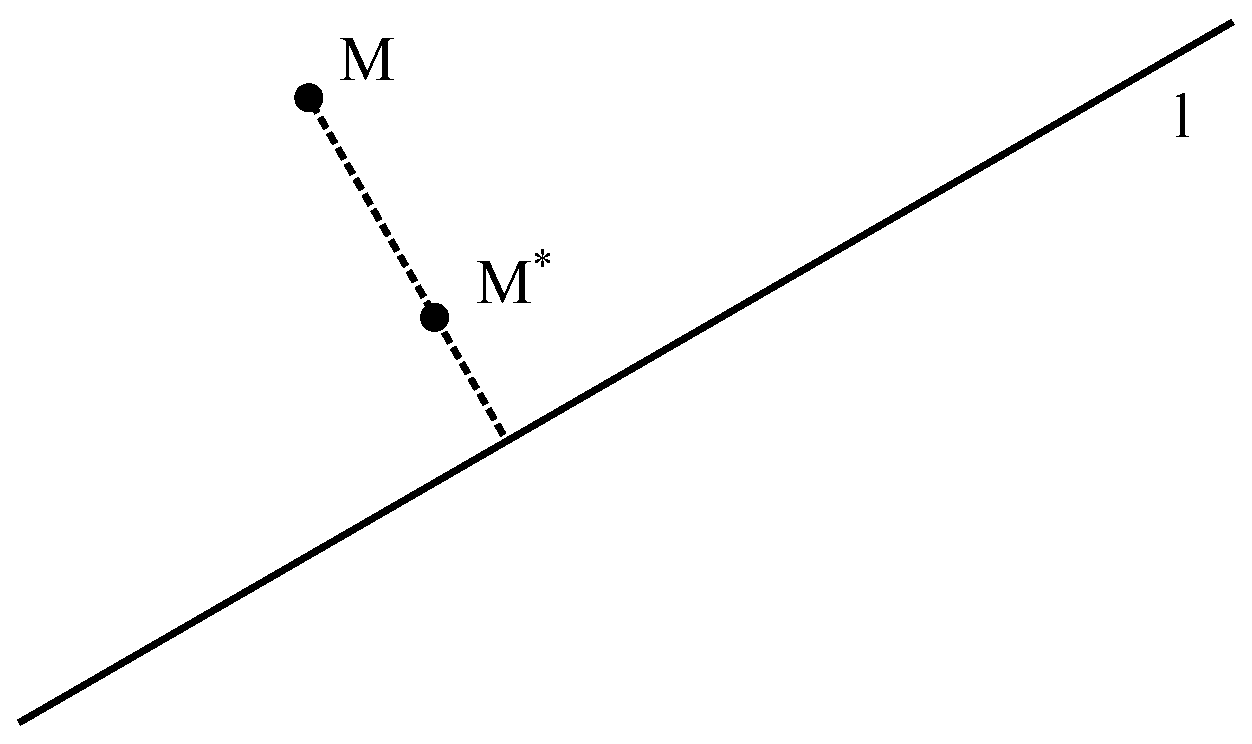
\includegraphics[width=0.5\columnwidth]{compressione-linea}
      
      \caption{Преобразование сжатия к прямой.}
      \label{fig:compressione-linea}
    \end{figure}
    
    Перейдём ко второму пункту задачи (про сжатие к прямой).
    Идея решения точно такая же: рассмотрим точку $M(x, y)$ и её образ $M^\star(x^\star, y^\star)$, получающийся в результате преобразования (\ref{fig:compressione-linea}).
    Суть сжатия к прямой $m$ с коэффициентом $k$ в том, что расстояния от точек до прямой $m$ изменяются в $k$ раз.
    При этом точка-образ $M^\star$ лежит на перпендикуляре из исходной точки к прямой, и по ту же сторону от прямой.
    Выпишем систему из упомянутых условий:
    \[
      \left\{
        \begin{aligned}
          &d(M^\star, m) = 2 \cdot d(M, m)\\
          &\vv{M M^\star} \perp m\\
        \end{aligned}
      \right.
    \]
    
    Расписывая через координаты, получаем
    \[
      \left\{
        \begin{aligned}
          &\frac{|2x^\star - y^\star + 5|}{\sqrt{2^2 + 1^2}} = 2 \cdot \frac{|2x - y + 5|}{\sqrt{2^2 + 1^2}}\\
          &(x^\star - x) \cdot 1 + (y^\star - y) \cdot 2 = 0\\
        \end{aligned}
      \right.
    \]
    
    Модули в первом уравнении системы \emph{раскрываются с одинаковыми знаками} (потому что обе точки лежат по одну сторону от прямой $m$, до которой вычисляется расстояние).
    Решая систему, находим координаты точки-образа $(x^\star, y^\star)$ через координаты исходной точки $(x, y)$...
  \end{solution}
  
  
  \subsection{\# 12.31}
  
  Доказать, что две касательные к эллипсу (или гиперболе) параллельны тогда и только тогда, когда точки касания и центр кривой лежат на одной прямой.
  
  \begin{solution}
    \begin{figure}
      \centering
      
      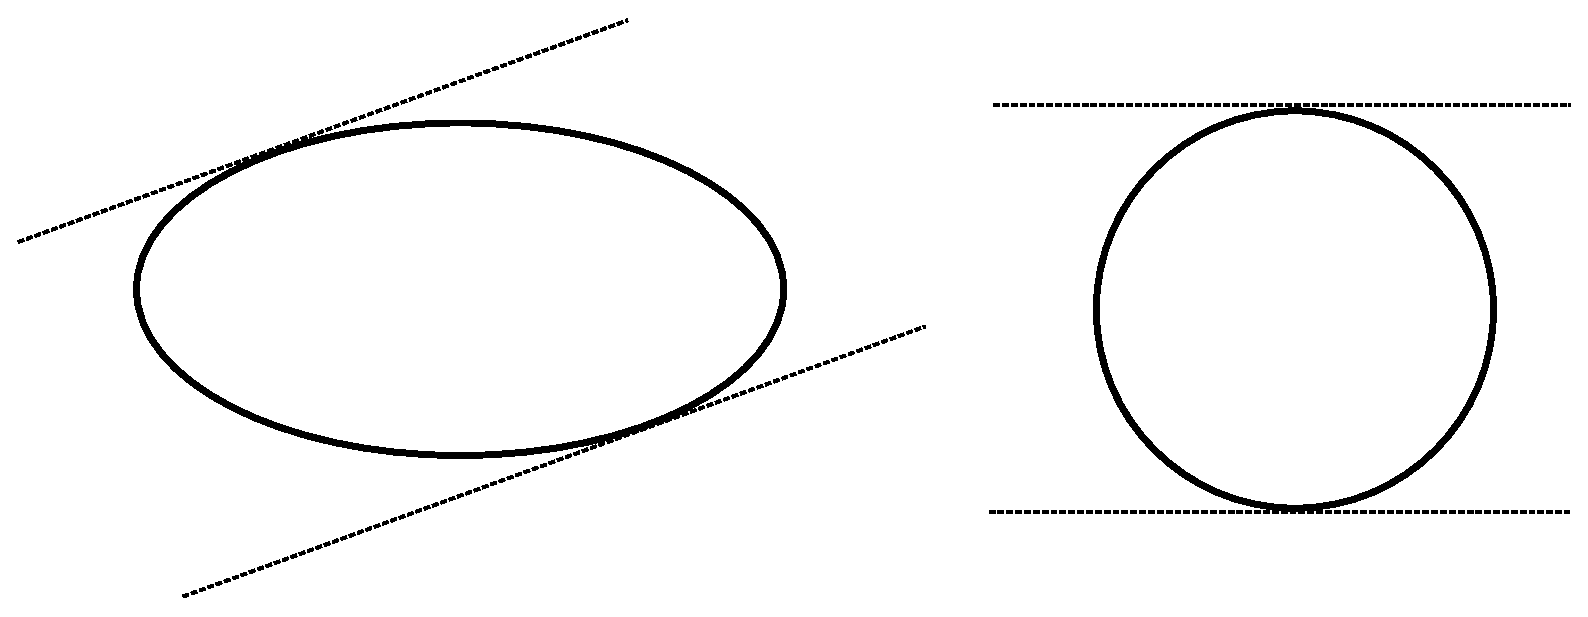
\includegraphics[width=0.5\columnwidth]{ellipse-new-ellipse}
      
      \caption{Отображение эллипса в окружность.}
      \label{fig:ellipse-new-ellipse}
    \end{figure}
    
    Рассмотрим сначала случай с эллипсом (\ref{fig:ellipse-new-ellipse}).
    Пусть две касательные к эллипсу параллельны.
    Обозначим точки касания за $A$ и $B$, а центр эллипса за $O$.
    Аффинным преобразованием переведём эллипс в окружность (для двух данных кривых второго порядка существует аффинное преобразование, которое переводит одну кривую в другую).
    При аффинном преобразовании прямая переходит в прямую, и параллельные прямые переходят в параллельные прямые.
    Поэтому образы параллельных касательных к эллипсу~---~параллельные касательные к окружности.
    Для окружности, очевидно, точки касания и центр будут лежать на одной прямой, точнее центр будет лежать не отрезке с концами в точках касания параллельных касательных.
    Обратным аффинным преобразованием переводим окружность обратно в эллипс.
    Отрезок при аффинном преобразовании переходит в отрезок, поэтому и в случае эллипса центр также будет лежать на отрезке с концами в касательных.
    
    Пусть точки касания эллипса лежат на одной прямой с центром эллипса.
    Аналогичным аффинным преобразованием можно перевести эллипс снова в окружность.
    При этом точки касания останутся на одной прямой с центром.
    Для окружности снова ``всё понятно''.
    Обратным преобразованием переводим окружность в эллипс, при этом параллельность прямых сохраняется.
    
    \bigskip

    %\begin{figure}
      %\centering
      %
      %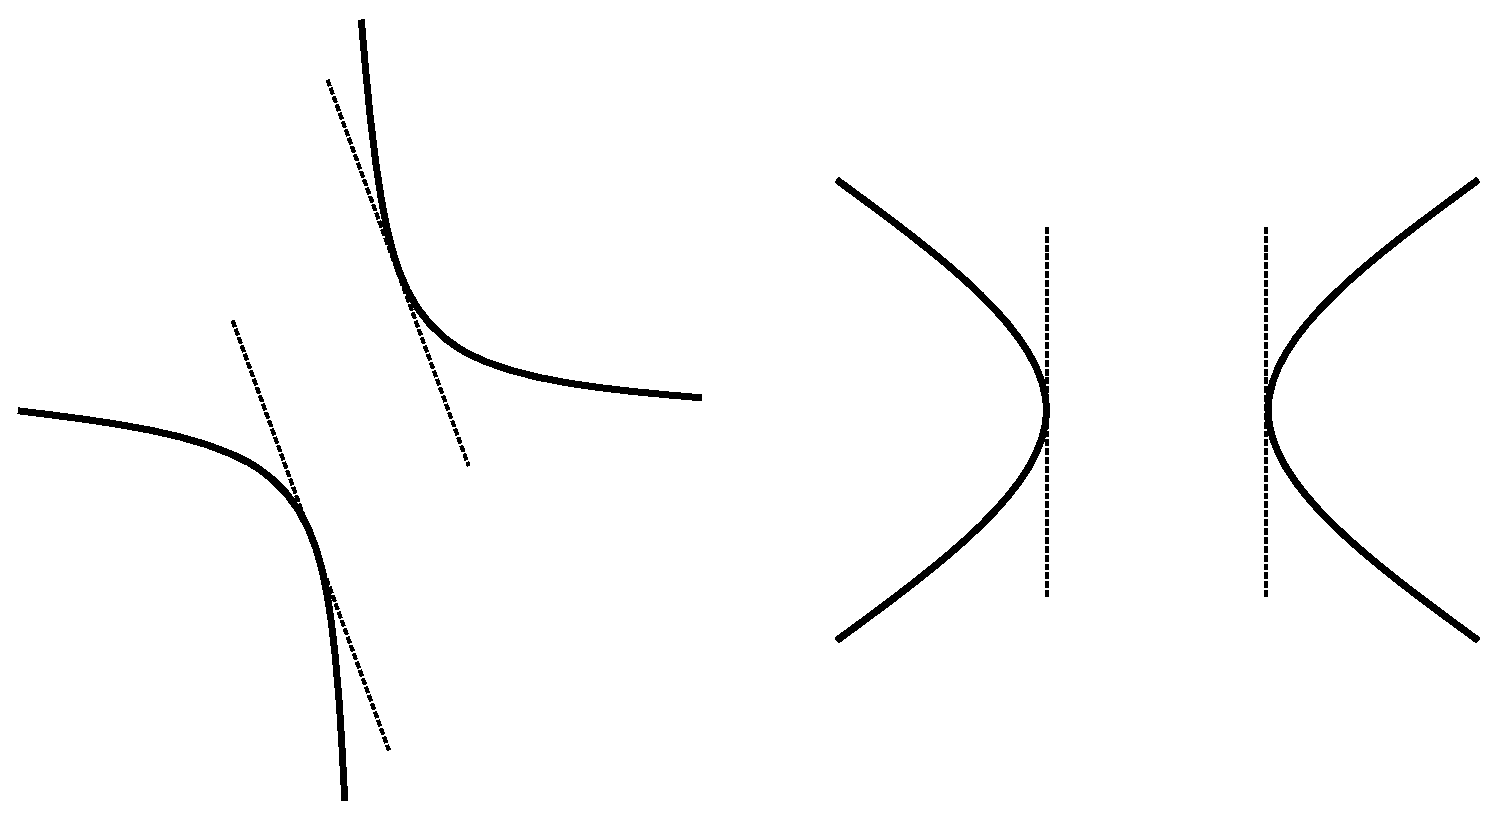
\includegraphics[width=0.5\columnwidth]{hyperbola-new-hyperbola}
      %
      %\caption{Отображение гиперболы в гиперболу: идея.}
      %\label{fig:hyperbola-new-hyperbola}
    %\end{figure}

    Для гиперболы всё ``в целом'' аналогично.
    Какой случай в случае гиперболы будет ``простым и понятным''?
    Для эллипса это была окружность.
    В какую гиперболу надо аффинным преобразованием переводить исходную?
    После возможных недолгих рассуждений можно прийти к выводу, что ``хорошей'' будет такая гипербола, у которой касательные проходят через вершины.
    Действительно, уж в таком случае всё более чем ``очевидно''.
    
    Сохраним обозначения для точек касания и для центра.
    Некоторым аффинным преобразованием можно исходную гиперболу перевести в ``хорошую''.
    Но как обеспечить то, чтоб точки касания перешли в вершины?..
    Аффинное преобразование однозначно задаётся образами трёх точек, не лежащих на одной прямой.
    Можем ли мы выбрать три ``подходящие'' точки, задающие нужное аффинное преобразование?
    Центр~$O$ можно перевести в центр~$O^*$.
    Точку касания~$A$ можно перевести в вершину ветви новой гиперболы~$A^*$.
    Вторую точку касания~$B$ можно перевести во вторую вершину~$B^*$?..
    Нет, это не очень хорошо.
    Потому, что точки $A$, $B$ и $O$ в условиях задачи лежат на одной прямой.
    С помощью них нельзя определить аффинное преобразование.
    Но никто не мешает выбрать ещё какую-нибудь точку гиперболы, отличную от точки~$B$.
    Пусть это будет некоторая точка $C$, например, \emph{с той же ветви, что и точка $B$}~(\ref{fig:from-hyperbola-to-hyperbola}).
    Как-нибудь выбираем образ~$C^*$.
    Как-нибудь, но \emph{именно с той же ветви образа гиперболы, на которой должна лежать точка $B^*$}.
    Аффинное преобразование задано.
    Исходные точки касания при этом переходят в вершины новой гиперболы.
    Далее уже всё просто.
    
    \begin{figure}
      \centering
      
      \includegraphics[width=0.8\columnwidth]{from-hyperbola-to-hyperbola}
      
      \caption{Отображение гиперболы в гиперболу.}  % Отображение гиперболы в гиперболу: задание ``конкретного'' преобразования.
      \label{fig:from-hyperbola-to-hyperbola}
    \end{figure}
    
    Пусть вначале касательные параллельны.
    Для ``новой'' гиперболы очевидно, что точки касания и центр лежат на одной прямой.
    Обратное преобразование, ..., точки касания и центр на одной прямой.
    
    Наоборот, пусть точки касания и центр лежат на одной прямой.
    Очевидно, касательные-образы параллельны.
    Обратное преобразование, ..., касательные параллельны.
  \end{solution}


  \subsection{\# 12.42(1)}
  
  Найти все неподвижные точки аффинного преобразования
  \[
    \left\{
      \begin{aligned}
        &x^* = 7x - 3y\\
        &y^* = x + y
      \end{aligned}
    \right.
  \]
  
  \begin{solution}
    \begin{definition}
      Неподвижная точка $(x, y)$ преобразования $f$~---~такая, которая под действием преобразования переходит в себя: $x^* \hm= x$, $y^* \hm= y$.
    \end{definition}
    
    То есть, чтобы найти неподвижные точки, надо решить систему
    \[
      \left\{
        \begin{aligned}
          &x = 7x - 3y\\
          &y = x + y
        \end{aligned}
      \right.
      \Leftrightarrow
      \left\{
        \begin{aligned}
          &6x - 3y = 0\\
          &x = 0
        \end{aligned}
      \right.
      \Leftrightarrow
      (x, y) = (0, 0)
    \]
  \end{solution}
  
  
  \subsection{\# 12.43(1) (``скетч'')}
  
  Найти инвариантные прямые линейного преобразования
  \[
    \left\{
      \begin{aligned}
        &x^* = 2x + 3y\\
        &y^* = -y
      \end{aligned}
    \right.
  \]
  
  \begin{solution}
    Приведём лишь начало решения.
    Основную ``смысловую'' часть.
    После которой, при желании, не сложно будет довести задачу до конца.
    
    Вспомним определение:
    
    \begin{definition}
      Множество точек $\mathcal M$ называется инвариантным относительно преобразования $f$, если все его точки под действием преобразования остаются в том же множестве, то есть $(x, y) \hm\in M \hm\Rightarrow (x^*, y^*) \hm\in M$.
    \end{definition}
    
    % TODO: ? для аффинного и "просто линейного"
    %\begin{remark}
      %Если $\mathcal M$ инвариантно, то ``стрелка в другую сторону'' может и ``не работать'':
      %\[
        %(x^*, y^*) \in M \xrightarrow{\?} (x, y) \in M
      %\]
      %то есть если образ лежит в $\mathcal M$, то прообраз не обязан вообще лежать в том же $\mathcal M$.
    %\end{remark}
    
    Будем искать инвариантную прямую $l$ в виде $Ax \hm+ By \hm+ C \hm= 0$.
    Тогда если точка $(x, y)$ лежит на прямой, то и её образ $(x^*, y^*)$ лежит на ней:
    \[
      \left\{
        \begin{aligned}
          &Ax + By + C = 0\\
          &Ax^* + By^* + C = 0
        \end{aligned}
      \right.
      \Leftrightarrow
      \left\{
        \begin{aligned}
          &Ax + By + C = 0\\
          &A\cdot (2x + 3y) + B\cdot (-y) + C = 0
        \end{aligned}
      \right.
      \Leftrightarrow
      \left\{
        \begin{aligned}
          &Ax + By + C = 0\\
          &2Ax + (3A - B)y + C = 0
        \end{aligned}
      \right.
    \]
    
    Что описывает второе уравнение системы?
    Прямую.
    Какую прямую?..
    Системе из \emph{двух} уравнений прямых удовлетворяет \emph{любая точка исходной прямой}.
    Значит, прямые, которые заданы первым и вторым уравнениями системы, должны описывать \emph{одну прямую}...
    
    Объяснить можно бы было и по-другому.
    Прямая, описываемая вторым уравнением~---~это \emph{прообраз образа} прямой~$l$.
    Так как мы имеем дело с аффинным преобразованием, то этот прообраз должен быть именно самой прямой~$l$.
    
    %\[
      %\frac{2A}{A} = \frac{3A - B}{B} = \frac{C}{C}
    %\]
    %
    %Далее надо рассмотреть несколько случаев.
    %Например, если $A \hm= 0$, то $\dfrac{-B}{B} \hm= \dfrac{C}{C}$.
    %При этом точно $B \hm{\not=} 0$.
    %Поэтому получаем $-1 \hm= \dfrac{C}{C}$, что в данной записи означает, что $C \hm= 0$.
    %Таким образом, первая инвариантная прямая (в качестве $B$ можно взять единицу):
    %\[
      %y = 0
    %\]
    %
    %Пусть теперь $A \hm{\not=} 0$.
    %Тогда получаем $2 \hm= \dfrac{3A - B}{B} = \dfrac{C}{C}$.
    %Снова получаем, что $C \hm= 0$.
    %Коэффициент $B$ находим из соотношения $2 \hm= \dfrac{3A - B}{B} \hm{\Leftrightarrow} 3A \hm- B \hm= 2B$.
    %Получается, что $B \hm= A$.
    %И уравнение инвариантной прямой (при $A \hm= 1$, например):
    %\[
      %x + y = 0
    %\]
    
  \end{solution}
  
  
  \subsection{\# 12.28(2) (``скетч'')}
  
  Доказать, что если аффинное преобразование~$f$ имеет единственную неподвижную точку, то все инвариантные прямые (если они существуют), проходят черех эту точку.
  
  \begin{solution}
    Приведём возможный ``план решения'' (``решение почти без спойлеров'').
    
    Первым делом, можно упростить себе жизнь, приняв неподвижную точку за начало системы координат.
    (Базис на всякий случай выбираем ``какой-нибудь'', но ортонормированный.)
    Какими формулами можно в таком случае (в выбранной системе координат) описать преобразование~$f$?
    
    Далее, что следует из того, что точка~$O$ (начало координат)~---~это \emph{единственная} неподвижная точка?
    Что это значит?
    Что из этого можно ``получить''?
    Как это ``переписать в других терминах''?)
    В терминах, связанных с преобразованием~$f$.
    
    Инвариантную прямую~$l$ снова можно искать в виде
    \[
      l\colon Ax + By + C = 0
    \]
    Когда эта прямая проходит через точку~$O$?
    Обязательно ли она через неё походит?
    Что будет, если допустить противное?
    Можно ли будет найти такую инвариантную прямую?
    
    Из ответов на поставленные вопросы и можно ``составить'' доказательство.
  \end{solution}
  
  
  \subsection{\# 12.82(6)}
  
  Представить аффинное преобразование $f$
  \[
    \left\{
      \begin{aligned}
        &x^* = 3y - 2\\
        &y^* = -4x
      \end{aligned}
    \right.
  \]
  в виде произведения
  \begin{equation}
    \label{eq:composition}
    f \hm= h_2 h_1 g
  \end{equation}
  где $g$~---~ортогональное преобразование, а $h_1$ и $h_2$~---~сжатия к двум взаимно перпендикулярным прямым.
  
  \begin{solution}
    Решение удобно начать с поиска \emph{главных} (сингулярных) направлений аффинного преобразования $f$: таких взаимно перпендикулярных направлений, которые под действием $f$ остаются взаимно перпендикулярными.
    Так как последними в композиции мы будем искать сжатия $h_1$ и $h_2$, то их можно будет искать как сжатия к образам некоторых прямых, параллельных главным направлениям, после ортогонального преобразования $g$.
    Главные направления $\bds u \hm= (\alpha_1, \beta_1)$ и $\bds v \hm= (\alpha_2, \beta_2)$ можно найти из системы:
    \[
      \left\{
        \begin{aligned}
          &\alpha_1 \alpha_2 + \beta_1 \beta_2 = 0\\
          &\alpha_1^* \alpha_2^* + \beta_1^* \beta_2^* = 0\\
          &\left\{
            \begin{aligned}
              &\alpha_1^* = 3\beta_1\\
              &\beta_1^* = -4\alpha_1\\
            \end{aligned}
          \right.
          \quad\left\{
            \begin{aligned}
              &\alpha_2^* = 3\beta_2\\
              &\beta_2^* = -4\alpha_2
            \end{aligned}
          \right.
        \end{aligned}
      \right.
    \]
    
    В итоге главными направлениями преобразования, например, будут
    \[
      \bds u = (0, 1),\quad \bds v = (1, 0)
    \]

    Ещё можно заметить, что определитель матрицы преобразования $f$:
    \[
      \Delta = \begin{vmatrix} 0 & 3\\ -4 & 0\end{vmatrix} = 12 > 0
    \]
    больше нуля, то есть образы базисных векторов будут образовывать на плоскости базис такой же ориентации, что и сам базис.
    Значит, в ортогональном преобразовании симметрия не потребуется.
    
    \begin{figure}
      \centering
      
      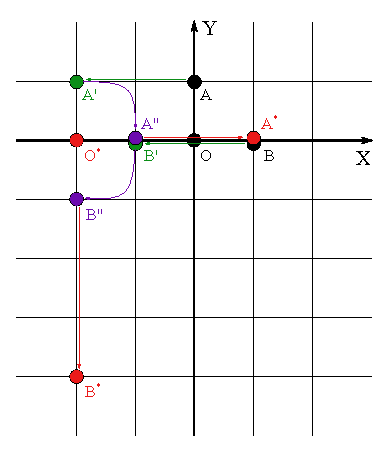
\includegraphics[width=0.5\columnwidth]{affine-as-composition}
      
      \caption{Аффинное преобразование как композиция ортогонального преобразования и сжатия к двум взаимно перпендикулярным прямым.}
      \label{fig:affine-as-composition}
    \end{figure}
    
    Теперь можно обратиться к картинке (\ref{fig:affine-as-composition}) и рассмотреть по шагам отображения трёх точек под действием $f$: точки-начала координат $O(0, 0)$, точки $A$, такой что $\vv{OA}$~---~главное направление $f$ (например, $A(0, 1)$), и точки $B$, такой что $\vv{OB}$~---~другое главное направление $f$ (например, $B(1, 0)$).
    Образы точек:
    \[
      \left\{
        \begin{aligned}
          &O(0, 0) \mapsto O^*(-2, 0)\\
          &A(0, 1) \mapsto A^*(1, 0)\\
          &B(1, 0) \mapsto B^*(-2, -4)
        \end{aligned}
      \right.
    \]
    
    Ортогональное преобразование $g$ из (\ref{eq:composition}) можно, в свою очередь, искать в виде композиции параллельного переноса, поворота и осевой симметрии (которой в данном случае, как выяснили ранее, не потребуется).
    В качестве параллельного переноса удобно сразу взять преобразование переноса на вектор $\vv{OO^*}$, так чтобы точка $O$, от которой отложены главные направления, перешла бы в свой образ под действием итогового $f$.
    Образы двух других точек после параллельного переноса обозначим за $A'$ и $B'$.
    Далее нужно будет повернуть все точки относительно $O^*$, так чтобы образ $A''$ точки $A$ под действием итогового $g$ оказался на луче $[O^*A^*)$ и образ $B''$ точки $B$ оказался бы на луче $[O^*B^*)$.
    Это будет поворот на угол $-\pi/2$ (на угол $\pi/2$ по часовой стрелке).
    И в конце можно найти коэффициенты сжатия к двум взаимно перпендикулярным прямым $O^*B^*$ и $O^*A^*$ как отношения $|O^*A^*|/|O^*A''|$ и $|O^*B^*|/|O^*B''|$ соответственно (которые окажутся равны $3$ и $4$).
    
    \emph{Стоит отметить, что система координат не меняется при преобразованиях! Меняются только координаты точек.}
    
    Можно ещё выписать формулы, задающие преобразования $g$, $h_1$ и $h_2$, и проверить, что их композиция в самом деле даёт $f$ (Обозначим за $g_1$ параллельный перенос и за $g_2$~---~поворот. Порядок сжатий вообще не важен.):
    \[
      \left\{
        \begin{aligned}
          &g_1\colon \left\{
            \begin{aligned}
              &x' = x - 2\\
              &y' = y
            \end{aligned}
          \right.\\
          &g_2\colon \left\{
            \begin{aligned}
              &x{''} = -2 + \bigl(x' - (-2)\bigr)\cos{\left(-\frac{\pi}{2}\right)} - (y' - 0)\sin{\left(-\frac{\pi}{2}\right)}\\
              &y{''} = 0 + \bigl(x' - (-2)\bigr)\sin{\left(-\frac{\pi}{2}\right)} + (y' - 0)\cos{\left(-\frac{\pi}{2}\right)}
            \end{aligned}
          \right.\\
          &h_1\colon \left\{
            \begin{aligned}
              &\bigl(x{'''} - (-2)\bigr)= 3 \cdot \bigl(x{''} - (-2)\bigr)\\
              &y{'''} = y{''}
            \end{aligned}
          \right.\\
          &h_2\colon \left\{
            \begin{aligned}
              &x^{\vartriangle} = x{'''}\\
              &(y^{\vartriangle} - 0) = 4 \cdot (y{'''} - 0)
            \end{aligned}
          \right.
        \end{aligned}
      \right.
    \]
    
    И в самом деле $f = h_2 \circ h_1 \circ \overbrace{g_2 \circ g_1}^g$:
    \[
      x^* = x^{\vartriangle},\quad y^* = x^{\vartriangle}
    \]
  \end{solution}

  
  
  \section{Ещё задача}
  
  
  \subsection{\# 12.26}
  
  Аффинное преобразование переводит три точки $A$, $B$, $C$, не лежащие на одной прямой, соответственно в точки $B$, $C$, $A$.
  Найти неподвижные точки этого преобразования.
  При каком необходимом и достаточном условии преобразование будет ортогональным\footnote{Ортогональное преобразование $f$~---~сохраняющее длины: $|AB| \hm= \bigr|f(A)f(B)\bigl|$. Так как вычисление длин в конечном итоге сводится к вычислению скалярных произведений между базисными векторами, то об ортогональном преобразовании можно думать и как о преобразовании, сохраняющем скалярные произведения.}?
  
  \begin{solution}
    Можно бы было решать задачу ``полностью'' координатным методом: ввести некоторую декартову систему координат на плоскости, через координаты точек $A$, $B$, и $C$ выразить коэффициенты аффинного преобразования и потом искать неподвижную точку как решение системы с, возможно, довольно громоздкими коэффициентами...
    
    Пойдём чуть более интеллектуальным путём.
    Три исходные точки не лежат на одной прямой.
    Значит, два из трёх векторов, которые можно построить на точках $A$, $B$ и $C$, можно взять в качестве базиса на плоскости.
    Зная образы базисных векторов, можно по ним разложить и любой вектор-образ\footnote{
      Образ вектора при аффинном преобразовании $f$ имеет в новом базисе те же координаты, что и исходный вектор в исходном базисе: $\bds v \hm= a \bds e_1 \hm+ b \bds e_2 \hm\Rightarrow f(\bds v) \hm= a f(\bds e_1) \hm+ b f(\bds e_2)$.
    }.
    Итак, предлагается выбрать векторы $\vv{AB} \hm\equiv \bds e_1$ и $\vv{BC} \hm\equiv \bds e_2$ в качестве базиса на плоскости.
    Образы базисных векторов:
    \[
      \left\{
        \begin{aligned}
          &\vv{AB} \mapsto \vv{BC}\\
          &\vv{BC} \mapsto \vv{CA}
        \end{aligned}
      \right.
    \]
    
    Обозначим образы базисных векторов за $\bds e_1'$ и $\bds e_2'$ и выразим их через исходные вектора
    \[
      \left\{
        \begin{aligned}
          &\bds e_1' = \vv{BC} = \bds e_2\\
          &\bds e_2' = \vv{CA} = \vv{CB} + \vv{BA} = -\bds e_2 - \bds e_1
        \end{aligned}
      \right.
    \]
    
    Мы хотим в итоге получить формулы для выражения координат $x'$, $y'$ точек через исходные координаты $x$, $y$.
    Для этого надо, наоборот, найти выражение \emph{исходных} базисных векторов через новые.
    Но это не сложно сделать:
    \[
      \left\{
        \begin{aligned}
          &\bds e_1 = -\bds e_1' - \bds e_2'\\
          &\bds e_2 = \bds e_1'
        \end{aligned}
      \right.
    \]
    
    Матрица перехода:
    \[
      S = \begin{pmatrix}-1 & 1\\ -1 & 0\end{pmatrix}
    \]
    
    Выражения для координат:
    \[
      \left\{
        \begin{aligned}
          &x^\star = -x + y + c_1\\
          &y^\star = -x + c_2
        \end{aligned}
      \right.
    \]
    
    \textbf{Но} перед тем, как писать выражения для координат, надо было выбрать начало системы координат (до этого были выбраны только базисные вектора).
    Для дальнейшего удобства решения предлагается выбрать начало не случайным, а равным, например, точке $A$.
    То есть полагаем $A(0, 0)$.
    
    Теперь можно выписать три системы из двух уравнений каждая для образов данных в условии задачи точек:
    \begin{equation}
      \label{eq:huge-system}
      \left\{
        \begin{aligned}
          &\left\{
            \begin{aligned}
              &x_A^\star = -x_A + y_A + c_1 = x_B\\
              &y_A^\star = -x_A + c_2 = y_B
            \end{aligned}
          \right.\\
          &\left\{
            \begin{aligned}
              &x_B^\star = -x_B + y_B + c_1 = x_C\\
              &y_B^\star = -x_B + c_2 = y_C
            \end{aligned}
          \right.\\
          &\left\{
            \begin{aligned}
              &x_C^\star = -x_C + y_C + c_1 = x_A\\
              &y_C^\star = -x_C + c_2 = y_A
            \end{aligned}
          \right.\\
        \end{aligned}
      \right.
    \end{equation}
    
    Из самой первой системы можно найти недостающие коэффициенты преобразования $c_1 \hm= x_B$ и $c_2 \hm= y_B$.
    Найдя эти коэффициенты, неподвижную точку можно найти как решение системы:
    \[
      \left\{
        \begin{aligned}
          &x = -x + y + c_1\\
          &y = -x + c_2
        \end{aligned}
      \right.
      \Leftrightarrow
      \left\{
        \begin{aligned}
          &x = \frac{c_1 + c_2}{3}\\
          &y = \frac{-c_1 + 2c_2}{3}
        \end{aligned}
      \right.
    \]
    
    То есть неподвижная точка получилась равной $\left(\dfrac{x_B + y_B}{3}, \dfrac{-x_B + 2y_B}{3}\right)$. На этом можно бы было, наверно, считать задачу решённой... но хоть ответ есть, он получился ``непонятный''.
    Чтобы ответ можно было ``потрогать'', надо получить выражения $x$ и $y$ компонент неподвижной точки через $x$ и $y$ компоненты точек из условия соответственно.
    Для этого надо вернуться к системе (\ref{eq:huge-system}) и выразить $c_1$ и $c_2$ по-другому.
    Можно бы было, наверное, сделать замену $c_1 \hm+ c_2$ и $-c_1 \hm+ 2c_2$~---~тогда бы было понятнее, что хочется получить при решении системы.
    Но можно и так (никаких подстановок делать не потребуется: надо просто выразить $c_1$ и $c_2$ из каждой из трёх систем и потом с этим ``играть'').
    В итоге координаты неподвижной точки:
    \[
      \left\{
        \begin{aligned}
          &x = \frac{(x_C + x_B - y_B) + (y_B)}{3} = \frac{x_B + x_C}{3}\\
          &y = \frac{-(y_B - y_C) + 2(y_B)}{3} = \frac{y_B + y_C}{3}
        \end{aligned}
      \right.
    \]
    
    Теперь понятно, что эта точка~---~точка пересечения медиан треугольника $ABC$!
    
    \bigskip
    
    Второй вопрос задачи кажется намного проще первого.
    Преобразование ортогональное, если оно сохраняет длины.
    Поэтому надо потребовать, чтобы длины образов базисных векторов были такими же, как и длины исходных векторов, и чтобы угол между образами был такой же, как и угол между прообразами.
    Условие на длины:
    \[
      \left\{
        \begin{aligned}
          &AB = BC\\
          &BC = CA
        \end{aligned}
      \right.
    \]
    означает, что треугольник $ABC$ равносторонний.
    При этом угол между образами базисных векторов тоже не меняется (остаётся равным $120\degree$).
  \end{solution}
  
  
  %\subsection{``Задача''}
  %
  %Для аффинного преобразования плоскости
  %\[
    %\left\{
      %\begin{aligned}
        %&x^\star = 6x - y + 2\\
        %&y^\star = 7x - 3y + 4
      %\end{aligned}
    %\right.
  %\]
  %надо найти
  %\begin{enumerate}
    %\item Площадь образа круга радиуса $1$
    %\item Площадь прообраза круга радиуса $1$
    %\item Все неподвижные точки
    %\item Все инвариантные прямые
  %\end{enumerate}
  %
  %\begin{solution}
    %Рассмотрим два неколлинеарных вектора $\bds u$ и $\bds v$.
    %Площадь параллелограмма, построенного на этих векторах:
    %\[
      %S_{\pm}(\bds u, \bds v) = \begin{vmatrix}u_1 & u_2\\ v_1 & v_2\end{vmatrix} \cdot S_{\pm}(\bds e_1, \bds e_2)
    %\]
    %
    %При аффинном преобразовании $f$ компоненты образов векторов в новом базисе получаются такими же, как в старом.
    %Поэтому для площади параллелограмма, построенного на векторах $\bds u^\star$ и $\bds v^\star$ верно
    %\[
      %S_{\pm}(\bds u^\star, \bds v^\star) = \begin{vmatrix}u_1 & u_2\\ v_1 & v_2\end{vmatrix} \cdot S_{\pm}\bigl(\bds e_1^\star, \bds e_2^\star\bigr)
      %= \begin{vmatrix}u_1 & u_2\\ v_1 & v_2\end{vmatrix} \begin{vmatrix}a_1 & a_2\\ b_1 & b_2\end{vmatrix} \cdot S_{\pm}(\bds e_1, \bds e_2)
    %\]
    %где в последнем переходе образы базисных векторов были выражены в исходном базисе.
%
    %Откуда отношение площади после преобразования к площади до преобразования:
    %\[
      %\frac{S^\star}{S} = \begin{vmatrix}a_1 & a_2\\ b_1 & b_2\end{vmatrix} = \begin{vmatrix}a_1 & b_1\\ a_2 & b_2\end{vmatrix}
    %\]
    %
    %Возвращаясь к задаче, отношение площадей по модулю будет равным
    %\[
      %\left|\det\begin{pmatrix}
        %6 & -1\\
        %7 & -3
      %\end{pmatrix}\right| = 11
    %\]
    %
    %Поэтому площадь образа круга радиуса $1$ будет равна $11 \pi\ \mbox{ед}^2$.
    %
    %Обратно, площадь прообраза круга радиуса $1$ будет равна $\dfrac{\pi}{11}\ \mbox{ед}^2$.
    %
    %Чтобы найти неподвижные точки преобразования, надо решить систему
    %\[
      %\left\{
        %\begin{aligned}
          %&x = 6x - y + 2\\
          %&y = 7x - 3y + 4
        %\end{aligned}
      %\right.
      %\Rightarrow \ldots
      %\Rightarrow \left\{
        %\begin{aligned}
          %&x = -\frac{4}{13}\\
          %&y = \frac{6}{13}
        %\end{aligned}
      %\right.
    %\]
    %
    %Инвариантные прямые можно искать в виде $Ax + By + C \hm= 0$.
    %Прямая $l$ инварианта относительно преобразования $f$, если $M \hm\in l \hm\Rightarrow M^\star \hm= f(M) \hm\in l$.
    %То есть
    %\begin{equation*}
    %\begin{split}
      %\left\{
        %\begin{aligned}
          %&Ax + By + C = 0\\
          %&Ax^\star + By^\star + C = 0
        %\end{aligned}
      %\right.
      %&\Leftrightarrow \left\{
        %\begin{aligned}
          %&Ax + By + C = 0\\
          %&A \cdot (6x - y + 2) + B \cdot (7x - 3y + 4) + C = 0
        %\end{aligned}
      %\right.\\
      %&\Leftrightarrow \left\{
        %\begin{aligned}
          %&Ax + By + C = 0\\
          %&(6A + 7B) x + (-A - 3B) y + (2A + 4B + C) = 0
        %\end{aligned}
      %\right.
    %\end{split}
    %\end{equation*}
    %
    %Получаем условие на коэффициенты преобразования
    %\[
      %\frac{6A + 7B}{A} = \frac{-A - 3B}{B} = \frac{2A + 4B + C}{C}
    %\]
    %
    %Решая получившуюся систему, и учитывая, что $A^2 \hm+ B^2 \hm> 0$, находим коэффициенты в уравнении прямых
    %\[
      %\left\{
        %\begin{aligned}
          %&A = B \cdot \left(-\frac{9}{2} \pm \frac{\sqrt{53}}{2}\right)\\
          %&C = B \cdot \left(-\frac{24}{13} \pm \frac{2\sqrt{53}}{13}\right)
        %\end{aligned}
      %\right.
    %\]
    %
    %И уравнения инвариантных прямых (при $B \hm= 26$):
    %\[
      %13\left(-9 \pm \sqrt{53}\right)x + 26y + 2\left(-24 \pm 2\sqrt{53}\right) = 0
    %\]
  %\end{solution}
  
  
  % TODO: в семинаре про определители: рассказать про производящие функции
\end{document}
